\documentclass[11pt]{article}
\usepackage[margin=1in]{geometry}
\usepackage{amsmath,amssymb}
\usepackage{graphicx}
\usepackage{booktabs}
\usepackage[colorlinks=true,linkcolor=blue,citecolor=blue,urlcolor=blue]{hyperref}

% --- the only two lines to edit before submission ---
\newcommand{\authorname}{Singularity}
\newcommand{\affiliation}{}

\title{Sparse L1 classification of medical abstracts\\ after removing duplicated and conflicting texts}
\author{\authorname\\ \small \affiliation}
\date{\today}

\begin{document}
\maketitle

\begin{abstract}
We ask whether an L1-penalised (LASSO) linear classifier gives a compact and accurate representation of medical
abstracts, a genuinely wide and sparse input. An audit of a public five-class corpus of 14,438 abstracts found 988
normalised texts shared between its supplied training and test files and 2,929 groups of identical texts, all with
conflicting labels. Keeping only unique, unambiguous abstracts left 8,298, which we split once (80/20). On the 1,660
held-out abstracts, LASSO reached a macro-F1 of 0.791 against 0.758 for ridge (L2) regression with the same features
and tuning; the paired difference was 0.033 (class-stratified bootstrap 95\% interval 0.014 to 0.053). LASSO used
2,201 of 250,000 class-specific coefficients (0.9\%), a few hundred readable terms per class. Probability ranking was
similar (macro AUC 0.952 against 0.956), so the gain lies in the class decisions.
\end{abstract}

\section{Introduction}
The LASSO~\cite{tibshirani1996} sets many coefficients exactly to zero and is widely used in health informatics for
variable selection. On tabular clinical records with a few dozen predictors its advantage over ridge regression is
often negligible, and a first test of ours on hospital readmission data found exactly that. Text is a different
setting: tens of thousands of word and phrase features, most of them irrelevant to any one class. We therefore ask
whether sparsity pays off where it has a direct job, choosing a small vocabulary that sorts abstracts into condition
groups, and whether that holds once repeated texts cannot leak between training and test.

\section{Methods}
\paragraph{Corpus audit.} The Medical Abstracts Text Classification Corpus~\cite{schopf2023,corpus} contains 11,550
training and 2,888 test rows labelled as neoplasms, digestive system diseases, nervous system diseases,
cardiovascular diseases or general pathological conditions. After case and whitespace normalisation, 988 texts
appeared in both supplied files, and 2,929 groups of identical texts carried more than one label. A repeated
abstract is not an independent test example and identical text with different labels cannot be resolved by a
single-label model, so every conflicting group was excluded and one record was kept per remaining text: 8,298
unique abstracts. The supplied split was not used.
\paragraph{Split and models.} One stratified 80/20 split (seed 20261107): 6,638 training and 1,660 test abstracts.
Features: TF--IDF unigrams and bigrams (minimum document frequency 2, at most 50,000 features, sublinear term
frequency, stop words kept so that negations remain). One-versus-rest logistic regression with an L1 (LASSO) or L2
(ridge) penalty, same solver; the inverse penalty $C\in\{0.03, 0.3, 3\}$ chosen for each by three-fold stratified
cross-validation on the training set only, maximising macro-F1. All choices were written down before modelling.
\paragraph{Measures.} Primary: held-out macro-F1 (equal weight to the five classes). Also accuracy, balanced
accuracy, macro one-versus-rest AUC and log loss; a class-stratified paired bootstrap (2,000 replicates) for the
LASSO-minus-ridge difference in macro-F1; overlap of the selected vocabularies across the three training folds.

\section{Results}
\begin{table}[h]
\centering
\begin{tabular}{lrrrrr}
\toprule
model & macro-F1 & accuracy & balanced acc. & macro AUC & log loss \\
\midrule
LASSO (L1) & \textbf{0.791} & \textbf{0.808} & \textbf{0.771} & 0.952 & 0.557 \\
ridge (L2) & 0.758 & 0.793 & 0.728 & \textbf{0.956} & 0.658 \\
\bottomrule
\end{tabular}
\caption{Held-out scores on 1,660 unique, unambiguous abstracts. Both penalties selected $C=3$.}
\label{tab:performance}
\end{table}

\begin{figure}[h]
\centering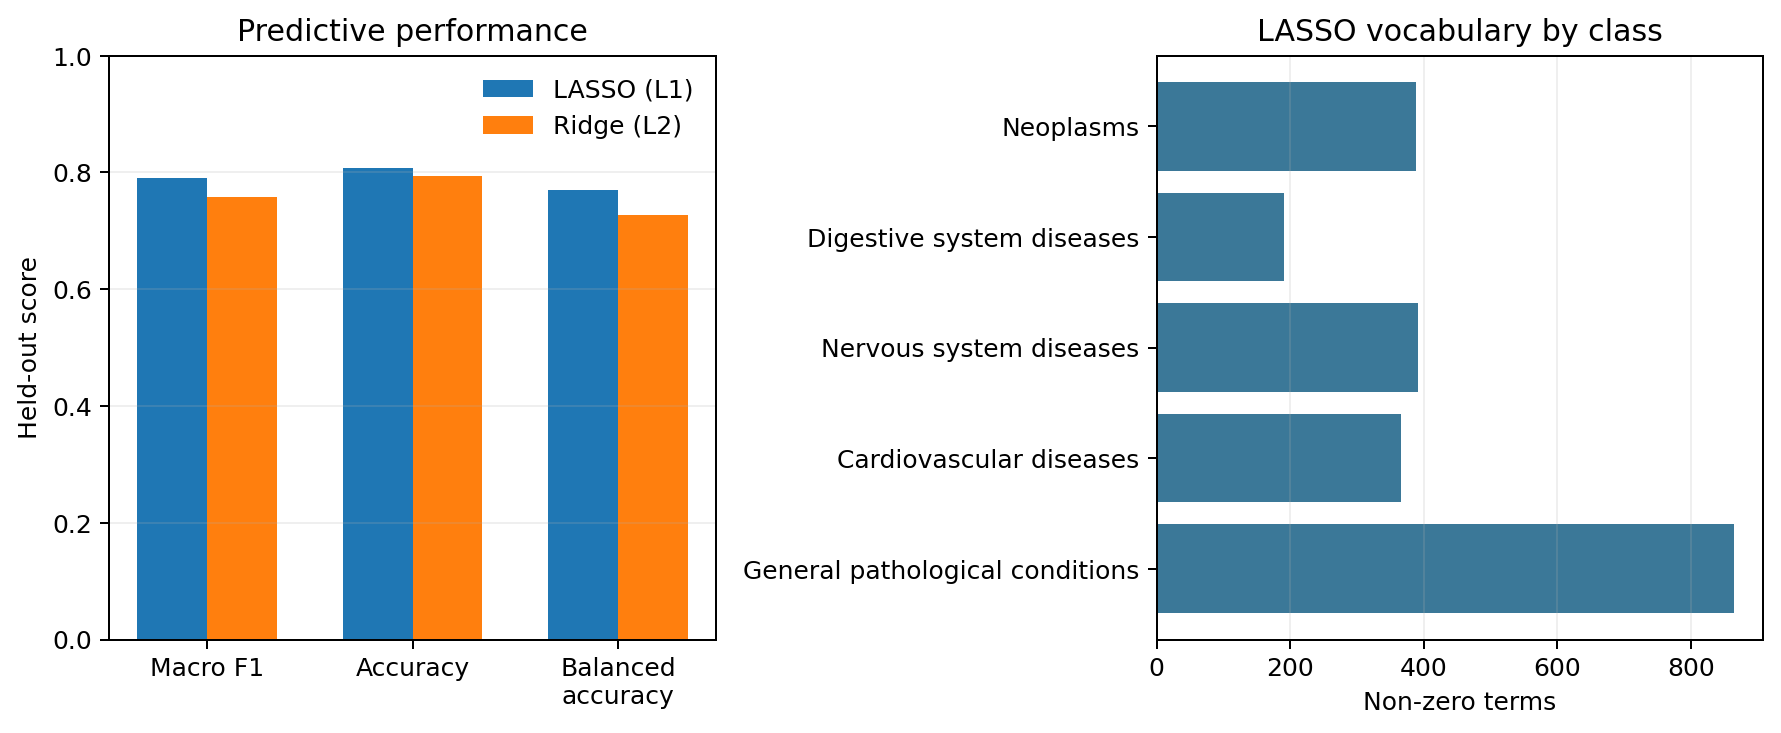
\includegraphics[width=.95\linewidth]{fig_results.png}
\caption{Left: held-out performance. Right: non-zero LASSO coefficients per class (2,201 in total).}
\label{fig:results}
\end{figure}

\begin{itemize}
\item \textbf{Better classification with fewer terms.} LASSO beat ridge by 0.033 in macro-F1 (interval 0.014 to
0.053), and also in accuracy and balanced accuracy, using 0.9\% of the coefficients.
\item \textbf{Compact vocabularies.} Between 190 terms (digestive system diseases) and 865 (general pathological
conditions) per class; the broad residual class needs the most words.
\item \textbf{Similar ranking.} Macro AUC was 0.952 against 0.956, so the advantage concerns hard class decisions
rather than probability ranking.
\item \textbf{Core vocabulary.} The mean pairwise Jaccard overlap of the selected vocabularies across three training
folds was 0.36: a shared part plus terms that change with the sample, which bagging could stabilise.
\end{itemize}

\section{Discussion}
In a high-dimensional text task, the L1 penalty both reduced the model to a few hundred terms per class and improved
the decisions that matter for sorting documents, in contrast with its near tie on tabular records. The audit is part of
the result: with the supplied split, nearly a thousand abstracts would have been scored on text seen in training, and
thousands of rows carry labels that contradict an identical copy. A compact, inspectable vocabulary is useful where
a classifier must be audited, and the same recipe can be applied to other clinical text collections.

\paragraph{Limitations.} One corpus, broad labels and a single holdout. The chosen penalty was at the edge of the
tested grid for both models, so a finer grid could change the margin. The selected words are associations with corpus
labels, not medical risk factors. Transformer models were not compared.

\paragraph{Reproducibility.} \texttt{experiment.py} runs the audit, split, tuning, evaluation, bootstrap and figure.
\texttt{results.json} contains the audit counts, the cross-validation grid, all held-out metrics with confusion
matrices, the bootstrap, sparsity and vocabulary overlap; the corpus is bundled under its CC BY-SA 3.0 licence.

\paragraph{Origin of the question.} The question came from an automated forecast (Singularity v3, registered on 5
November 2026 with a SHA-256 fingerprint, view of classic methods) that LASSO regression would enter the subfield \emph{Health Informatics}.
The forecast concerned the arrival of the method, not the result of this study.

\begin{thebibliography}{9}
\bibitem{tibshirani1996} R.~Tibshirani, Regression shrinkage and selection via the lasso, \emph{Journal of the Royal
Statistical Society B} 58, 267--288 (1996).
\bibitem{schopf2023} T.~Schopf, D.~Braun and F.~Matthes, Evaluating unsupervised text classification: zero-shot and
similarity-based approaches, \emph{Proc.\ 6th International Conference on Natural Language Processing and Information
Retrieval}, 6--15 (2023), doi:10.1145/3582768.3582795.
\bibitem{corpus} T.~Schopf, D.~Braun and F.~Matthes, Medical Abstracts Text Classification Corpus,
github.com/sebischair/Medical-Abstracts-TC-Corpus, CC BY-SA 3.0.
\end{thebibliography}
\end{document}
